
%% bare_conf.tex
%% V1.4a
%% 2014/09/17
%% by Michael Shell
%% See:
%% http://www.michaelshell.org/
%% for current contact information.
%%
%% This is a skeleton file demonstrating the use of IEEEtran.cls
%% (requires IEEEtran.cls version 1.8a or later) with an IEEE
%% conference paper.
%%
%% Support sites:
%% http://www.michaelshell.org/tex/ieeetran/
%% http://www.ctan.org/tex-archive/macros/latex/contrib/IEEEtran/
%% and
%% http://www.ieee.org/

%%*************************************************************************
%% Legal Notice:
%% This code is offered as-is without any warranty either expressed or
%% implied; without even the implied warranty of MERCHANTABILITY or
%% FITNESS FOR A PARTICULAR PURPOSE! 
%% User assumes all risk.
%% In no event shall IEEE or any contributor to this code be liable for
%% any damages or losses, including, but not limited to, incidental,
%% consequential, or any other damages, resulting from the use or misuse
%% of any information contained here.
%%
%% All comments are the opinions of their respective authors and are not
%% necessarily endorsed by the IEEE.
%%
%% This work is distributed under the LaTeX Project Public License (LPPL)
%% ( http://www.latex-project.org/ ) version 1.3, and may be freely used,
%% distributed and modified. A copy of the LPPL, version 1.3, is included
%% in the base LaTeX documentation of all distributions of LaTeX released
%% 2003/12/01 or later.
%% Retain all contribution notices and credits.
%% ** Modified files should be clearly indicated as such, including  **
%% ** renaming them and changing author support contact information. **
%%
%% File list of work: IEEEtran.cls, IEEEtran_HOWTO.pdf, bare_adv.tex,
%%                    bare_conf.tex, bare_jrnl.tex, bare_conf_compsoc.tex,
%%                    bare_jrnl_compsoc.tex, bare_jrnl_transmag.tex
%%*************************************************************************


% *** Authors should verify (and, if needed, correct) their LaTeX system  ***
% *** with the testflow diagnostic prior to trusting their LaTeX platform ***
% *** with production work. IEEE's font choices and paper sizes can       ***
% *** trigger bugs that do not appear when using other class files.       ***                          ***
% The testflow support page is at:
% http://www.michaelshell.org/tex/testflow/



\documentclass[conference]{IEEEtran}
% Some Computer Society conferences also require the compsoc mode option,
% but others use the standard conference format.
%
% If IEEEtran.cls has not been installed into the LaTeX system files,
% manually specify the path to it like:
% \documentclass[conference]{../sty/IEEEtran}





% Some very useful LaTeX packages include:
% (uncomment the ones you want to load)


% *** MISC UTILITY PACKAGES ***
%
%\usepackage{ifpdf}
% Heiko Oberdiek's ifpdf.sty is very useful if you need conditional
% compilation based on whether the output is pdf or dvi.
% usage:
% \ifpdf
%   % pdf code
% \else
%   % dvi code
% \fi
% The latest version of ifpdf.sty can be obtained from:
% http://www.ctan.org/tex-archive/macros/latex/contrib/oberdiek/
% Also, note that IEEEtran.cls V1.7 and later provides a builtin
% \ifCLASSINFOpdf conditional that works the same way.
% When switching from latex to pdflatex and vice-versa, the compiler may
% have to be run twice to clear warning/error messages.






% *** CITATION PACKAGES ***
%
%\usepackage{cite}
% cite.sty was written by Donald Arseneau
% V1.6 and later of IEEEtran pre-defines the format of the cite.sty package
% \cite{} output to follow that of IEEE. Loading the cite package will
% result in citation numbers being automatically sorted and properly
% "compressed/ranged". e.g., [1], [9], [2], [7], [5], [6] without using
% cite.sty will become [1], [2], [5]--[7], [9] using cite.sty. cite.sty's
% \cite will automatically add leading space, if needed. Use cite.sty's
% noadjust option (cite.sty V3.8 and later) if you want to turn this off
% such as if a citation ever needs to be enclosed in parenthesis.
% cite.sty is already installed on most LaTeX systems. Be sure and use
% version 5.0 (2009-03-20) and later if using hyperref.sty.
% The latest version can be obtained at:
% http://www.ctan.org/tex-archive/macros/latex/contrib/cite/
% The documentation is contained in the cite.sty file itself.






% *** GRAPHICS RELATED PACKAGES ***
%
\ifCLASSINFOpdf
  \usepackage[pdftex]{graphicx}
%   declare the path(s) where your graphic files are
  \graphicspath{{Figs/}}
  % and their extensions so you won't have to specify these with
  % every instance of \includegraphics
  \DeclareGraphicsExtensions{.pdf,.jpeg,.png}
\else
  % or other class option (dvipsone, dvipdf, if not using dvips). graphicx
  % will default to the driver specified in the system graphics.cfg if no
  % driver is specified.
  % \usepackage[dvips]{graphicx}
  % declare the path(s) where your graphic files are
  % \graphicspath{{../eps/}}
  % and their extensions so you won't have to specify these with
  % every instance of \includegraphics
  % \DeclareGraphicsExtensions{.eps}
\fi
% graphicx was written by David Carlisle and Sebastian Rahtz. It is
% required if you want graphics, photos, etc. graphicx.sty is already
% installed on most LaTeX systems. The latest version and documentation
% can be obtained at: 
% http://www.ctan.org/tex-archive/macros/latex/required/graphics/
% Another good source of documentation is "Using Imported Graphics in
% LaTeX2e" by Keith Reckdahl which can be found at:
% http://www.ctan.org/tex-archive/info/epslatex/
%
% latex, and pdflatex in dvi mode, support graphics in encapsulated
% postscript (.eps) format. pdflatex in pdf mode supports graphics
% in .pdf, .jpeg, .png and .mps (metapost) formats. Users should ensure
% that all non-photo figures use a vector format (.eps, .pdf, .mps) and
% not a bitmapped formats (.jpeg, .png). IEEE frowns on bitmapped formats
% which can result in "jaggedy"/blurry rendering of lines and letters as
% well as large increases in file sizes.
%
% You can find documentation about the pdfTeX application at:
% http://www.tug.org/applications/pdftex





% *** MATH PACKAGES ***
%
%\usepackage[cmex10]{amsmath}
% A popular package from the American Mathematical Society that provides
% many useful and powerful commands for dealing with mathematics. If using
% it, be sure to load this package with the cmex10 option to ensure that
% only type 1 fonts will utilized at all point sizes. Without this option,
% it is possible that some math symbols, particularly those within
% footnotes, will be rendered in bitmap form which will result in a
% document that can not be IEEE Xplore compliant!
%
% Also, note that the amsmath package sets \interdisplaylinepenalty to 10000
% thus preventing page breaks from occurring within multiline equations. Use:
%\interdisplaylinepenalty=2500
% after loading amsmath to restore such page breaks as IEEEtran.cls normally
% does. amsmath.sty is already installed on most LaTeX systems. The latest
% version and documentation can be obtained at:
% http://www.ctan.org/tex-archive/macros/latex/required/amslatex/math/





% *** SPECIALIZED LIST PACKAGES ***
%
%\usepackage{algorithmic}
% algorithmic.sty was written by Peter Williams and Rogerio Brito.
% This package provides an algorithmic environment fo describing algorithms.
% You can use the algorithmic environment in-text or within a figure
% environment to provide for a floating algorithm. Do NOT use the algorithm
% floating environment provided by algorithm.sty (by the same authors) or
% algorithm2e.sty (by Christophe Fiorio) as IEEE does not use dedicated
% algorithm float types and packages that provide these will not provide
% correct IEEE style captions. The latest version and documentation of
% algorithmic.sty can be obtained at:
% http://www.ctan.org/tex-archive/macros/latex/contrib/algorithms/
% There is also a support site at:
% http://algorithms.berlios.de/index.html
% Also of interest may be the (relatively newer and more customizable)
% algorithmicx.sty package by Szasz Janos:
% http://www.ctan.org/tex-archive/macros/latex/contrib/algorithmicx/




% *** ALIGNMENT PACKAGES ***
%
%\usepackage{array}
% Frank Mittelbach's and David Carlisle's array.sty patches and improves
% the standard LaTeX2e array and tabular environments to provide better
% appearance and additional user controls. As the default LaTeX2e table
% generation code is lacking to the point of almost being broken with
% respect to the quality of the end results, all users are strongly
% advised to use an enhanced (at the very least that provided by array.sty)
% set of table tools. array.sty is already installed on most systems. The
% latest version and documentation can be obtained at:
% http://www.ctan.org/tex-archive/macros/latex/required/tools/


% IEEEtran contains the IEEEeqnarray family of commands that can be used to
% generate multiline equations as well as matrices, tables, etc., of high
% quality.




% *** SUBFIGURE PACKAGES ***
%\ifCLASSOPTIONcompsoc
%  \usepackage[caption=false,font=normalsize,labelfont=sf,textfont=sf]{subfig}
%\else
%  \usepackage[caption=false,font=footnotesize]{subfig}
%\fi
% subfig.sty, written by Steven Douglas Cochran, is the modern replacement
% for subfigure.sty, the latter of which is no longer maintained and is
% incompatible with some LaTeX packages including fixltx2e. However,
% subfig.sty requires and automatically loads Axel Sommerfeldt's caption.sty
% which will override IEEEtran.cls' handling of captions and this will result
% in non-IEEE style figure/table captions. To prevent this problem, be sure
% and invoke subfig.sty's "caption=false" package option (available since
% subfig.sty version 1.3, 2005/06/28) as this is will preserve IEEEtran.cls
% handling of captions.
% Note that the Computer Society format requires a larger sans serif font
% than the serif footnote size font used in traditional IEEE formatting
% and thus the need to invoke different subfig.sty package options depending
% on whether compsoc mode has been enabled.
%
% The latest version and documentation of subfig.sty can be obtained at:
% http://www.ctan.org/tex-archive/macros/latex/contrib/subfig/




% *** FLOAT PACKAGES ***
%
%\usepackage{fixltx2e}
% fixltx2e, the successor to the earlier fix2col.sty, was written by
% Frank Mittelbach and David Carlisle. This package corrects a few problems
% in the LaTeX2e kernel, the most notable of which is that in current
% LaTeX2e releases, the ordering of single and double column floats is not
% guaranteed to be preserved. Thus, an unpatched LaTeX2e can allow a
% single column figure to be placed prior to an earlier double column
% figure. The latest version and documentation can be found at:
% http://www.ctan.org/tex-archive/macros/latex/base/


%\usepackage{stfloats}
% stfloats.sty was written by Sigitas Tolusis. This package gives LaTeX2e
% the ability to do double column floats at the bottom of the page as well
% as the top. (e.g., "\begin{figure*}[!b]" is not normally possible in
% LaTeX2e). It also provides a command:
%\fnbelowfloat
% to enable the placement of footnotes below bottom floats (the standard
% LaTeX2e kernel puts them above bottom floats). This is an invasive package
% which rewrites many portions of the LaTeX2e float routines. It may not work
% with other packages that modify the LaTeX2e float routines. The latest
% version and documentation can be obtained at:
% http://www.ctan.org/tex-archive/macros/latex/contrib/sttools/
% Do not use the stfloats baselinefloat ability as IEEE does not allow
% \baselineskip to stretch. Authors submitting work to the IEEE should note
% that IEEE rarely uses double column equations and that authors should try
% to avoid such use. Do not be tempted to use the cuted.sty or midfloat.sty
% packages (also by Sigitas Tolusis) as IEEE does not format its papers in
% such ways.
% Do not attempt to use stfloats with fixltx2e as they are incompatible.
% Instead, use Morten Hogholm'a dblfloatfix which combines the features
% of both fixltx2e and stfloats:
%
% \usepackage{dblfloatfix}
% The latest version can be found at:
% http://www.ctan.org/tex-archive/macros/latex/contrib/dblfloatfix/




% *** PDF, URL AND HYPERLINK PACKAGES ***
%
%\usepackage{url}
% url.sty was written by Donald Arseneau. It provides better support for
% handling and breaking URLs. url.sty is already installed on most LaTeX
% systems. The latest version and documentation can be obtained at:
% http://www.ctan.org/tex-archive/macros/latex/contrib/url/
% Basically, \url{my_url_here}.




% *** Do not adjust lengths that control margins, column widths, etc. ***
% *** Do not use packages that alter fonts (such as pslatex).         ***
% There should be no need to do such things with IEEEtran.cls V1.6 and later.
% (Unless specifically asked to do so by the journal or conference you plan
% to submit to, of course. )


% correct bad hyphenation here
\hyphenation{op-tical net-works semi-conduc-tor}


\begin{document}
%
% paper title
% Titles are generally capitalized except for words such as a, an, and, as,
% at, but, by, for, in, nor, of, on, or, the, to and up, which are usually
% not capitalized unless they are the first or last word of the title.
% Linebreaks \\ can be used within to get better formatting as desired.
% Do not put math or special symbols in the title.
\title{Watermelon Project - Team Description Paper RoCKIn@home 2015}


% author names and affiliations
% use a multiple column layout for up to three different
% affiliations
\author{\IEEEauthorblockN{Francisco J. Rodr\'iguez Lera, Fernando Casado, Vicente Matell\'an}
\IEEEauthorblockA{%School of Electrical and Computer Engineering\\
University of Le\'on\\
Campus de Vegazana, s/n, Le\'on, Spain\\
Email: http://robotica.unileon.es}
\and
\IEEEauthorblockN{Francisco Mart\'in }
\IEEEauthorblockA{Universidad Rey Juan Carlos\\
Fuenlabrada, Madrid, Spain\\
Email: http://robotica.gsyc.es}}
% \and
% \IEEEauthorblockN{James Kirk\\ and Montgomery Scott}
% \IEEEauthorblockA{Starfleet Academy\\
% San Francisco, California 96678--2391\\
% Telephone: (800) 555--1212\\
% Fax: (888) 555--1212}}

% conference papers do not typically use \thanks and this command
% is locked out in conference mode. If really needed, such as for
% the acknowledgment of grants, issue a \IEEEoverridecommandlockouts
% after \documentclass

% for over three affiliations, or if they all won't fit within the width
% of the page, use this alternative format:
% 
%\author{\IEEEauthorblockN{Michael Shell\IEEEauthorrefmark{1},
%Homer Simpson\IEEEauthorrefmark{2},
%James Kirk\IEEEauthorrefmark{3}, 
%Montgomery Scott\IEEEauthorrefmark{3} and
%Eldon Tyrell\IEEEauthorrefmark{4}}
%\IEEEauthorblockA{\IEEEauthorrefmark{1}School of Electrical and Computer Engineering\\
%Georgia Institute of Technology,
%Atlanta, Georgia 30332--0250\\ Email: see http://www.michaelshell.org/contact.html}
%\IEEEauthorblockA{\IEEEauthorrefmark{2}Twentieth Century Fox, Springfield, USA\\
%Email: homer@thesimpsons.com}
%\IEEEauthorblockA{\IEEEauthorrefmark{3}Starfleet Academy, San Francisco, California 96678-2391\\
%Telephone: (800) 555--1212, Fax: (888) 555--1212}
%\IEEEauthorblockA{\IEEEauthorrefmark{4}Tyrell Inc., 123 Replicant Street, Los Angeles, California 90210--4321}}




% use for special paper notices
%\IEEEspecialpapernotice{(Invited Paper)}




% make the title area
\maketitle

% in the abstract
\begin{abstract}
This document describes the developments of \textit{Watermelon Project} team for the participation in the RoCKIn@home challenge, that will take place in Lisbon in November 2015. 
This Team Description Paper (TDP) describes: the team trajectory and the relevant research lines for facing the tasks of this competition.
From the hardware point of view, we introduce here our RB1 platform designed and manufactured by Robotnik. We review its main characteristics and the capabilities for addressing service and assistive tasks.
Attending the software solutions, we present here our contributions to face assistive tasks in home-like environments. 
This paper presents our preliminary results prior the competition.
\end{abstract}

% no keywords




% For peer review papers, you can put extra information on the cover
% page as needed:
% \ifCLASSOPTIONpeerreview
% \begin{center} \bfseries EDICS Category: 3-BBND \end{center}
% \fi
%
% For peerreview papers, this IEEEtran command inserts a page break and
% creates the second title. It will be ignored for other modes.
\IEEEpeerreviewmaketitle



\section{Introduction}

Watermelon Project team was originally created by the group of robotics at the University of
Le\'on in 2012. In 2013 it was expanded with the addition of Robotics Group at the Rey Juan
Carlos University. 

Our original goal was to prove that a robotic platform could be created  using low-cost materials.
We wanted to validate it as a starter kit for robotics researchers in competitions like RoCKIn or other
endeavours. The RoCKIn 2014 events allowed us to test our approach intensively, and introduce
several improvements and fixes in our robot. Finally, we have concluded that 
this robot can be used in the labs for researching and for analyzing semi-autonomous behaviours in 
real homes. 

MYRA (“Elderly and Augmented Reality” in Spanish) was the code name given to the original
project more than two years ago. The main goal was to build an assistance robotics platform
that would be suited to the needs of old people, such as helping them to take the right
medication at the right time. We intended to study the human-robot interaction using
augmented reality, and a target demographic with usually little experience with robots or
technology overall. The Watermelon team was formed at the end of 2013, in order to
participate in the RoCKIn@Home camp that was going to take place in Rome on January the
next year. Since the first moment, we focused our efforts on adding new software and
hardware solutions, or improving the existing ones, in order to adapt MYRA for the
competition. Thus the MYRABot platform was created, and it has been continuously reshaped
ever since.

\begin{figure}[ht]
  \centering
  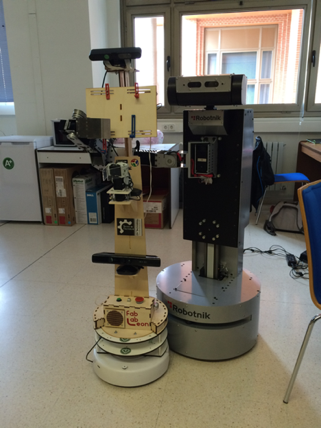
\includegraphics[width=0.3\textwidth]{179}
  \caption{MYRABot and RB-1 Robots} 
  \label{fig:robots1}
\end{figure}



With the robotic platform MYRABot we have participated in all the events organized by
RoCKIn. For this final event, also we plan to test our algorithms in the robotics platform
RB-1, which is more robust and advanced than MYRABot. Figure~\ref{fig:robots1} shows both robots in our lab.



Throughout this document we will enumerate the current features of MYRABot and RB-1,
including the improvements that have been integrated since the last RoCKIn event that took
place in Toulouse last November.

The paper is organized as follows: Section~\ref{sec:teamdescription} reviews our experience in robotics competitions and a brief description of team members. Section~\ref{sec:hardwaredescription} introduces our new robot RB1 and highlights its hardware characteristics. Section~\ref{sec:softwaredescription} focus on the software solutions implemented to our platform. The next section presents our RoCKIn plan and the safety requirements of our platform. Finally section~\ref{sec:conclusions} presents the conclusions of our RoCKIn approach. 



\begin{figure*}[t!]
  \centering
  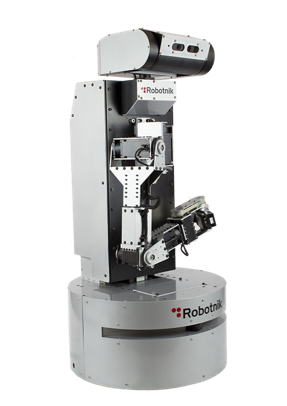
\includegraphics[width=0.25\textwidth]{21113}
  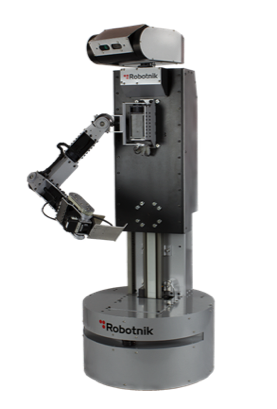
\includegraphics[width=0.25\textwidth]{31177}
  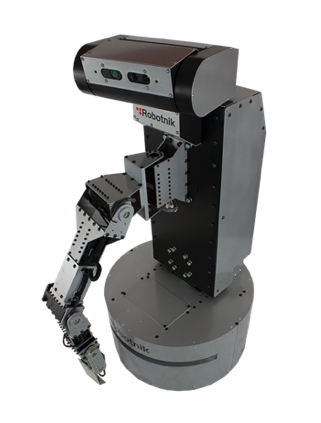
\includegraphics[width=0.25\textwidth]{91195}
  \caption{RB-1 Robot} 
  \label{fig:robots}
\end{figure*}


\section{Team Description}
\label{sec:teamdescription}

The Watermelon Project team is composed by members with previous experience in robotic competitions. 
Before participating in RoCKIn, they have been involved in the RoboCup Competition, in the 4-legged League and the Standard Platform League (SPL). 
They have been participating in these competitions since RoboCup 2005, which took place in Osaka (Japan) until RoboCup 2011.
The Watermelon Project team was born with a small roster of MSc and Ph.D. students from the ULE robotics group, mainly.

Watermelon Project team has participated in all previous RoCKIn editions: a) Camp Eindhoven 2013,  b) Camp Rome 2013, c) Competition Toulouse 2014, and d) Camp Peccioli 2013.
% \begin{itemize}
%   \item RoCKIn Camp Eindhoven 2013
%   \item RoCKIn Camp Rome 2013
%   \item RoCKIn Competition Toulouse 2014
%   \item RoCKIn Camp Peccioli 2013
% \end{itemize}

During this process, we have published different scientific contributions associated with the evolution of our MYRABot platform~\cite{lera2014mobile},\cite{martin2014myrabot},~\cite{lera2014building}.




\subsection{Team Members}

\textbf{Francisco Lera} is a Ph.D. student in Universidad de Le\'on, creator of MYRABot and prime mover of the project. 

\textbf{Fernando Casado} is a Ph.D. student specialized in electronics and hardware, and currently manipulation and grasping

\textbf{Francisco Mart\'in Rico} is a Ph.D. from Rey Juan Carlos University (URJC), with a long experience in robotics competitions such as RoboCup SPL. His many
contributions include the behaviour  control system.

\textbf{Vicente Matell\'an} is a Professor in Universidad de Le\'on. Overseer and leader of the ULE Robotics Group.


% % % % % % % % % % % % % % % % % % % % % % 
% % % % % % % % % % % % % % % % % % % % % % 
\section{Robot Hardware Description}
\label{sec:hardwaredescription}

% % % % % % % % % % % % % % % % % % % % % % 
We plan to attend the RoCKIn@Home challenge in  Lisbon  with  RB1  robot (Fig.~\ref{fig:robots}). 
The platform is a mobile manipulator designed and manufacture by Robotnik~\cite{Robotnik2015,IEEESpectrum2015}. 
The Technical specification document\cite{TechnicalRobotnik2015} enumerates its main physical characteristics.


% 
% The robot has been designed using a single type of the korean manufacturer ROBOTIS actuators and corresponding with the product range Dynamixel PRO. 
% % The design is modular and scalable. 
% The Dynamixel PRO servo-actuators integrate controller and servo-amplifier inside the actuator housing, simplifying its interconnection to 2 supply wires and 2 additional wires for a communication bus. 
% This kind of actuators has been successfully used in robots as Thor-op, one of the humanoids that took part in the last DARPA Grand Challenge.


RB1 mobile platform  has a differential drive steering.  
The platform mounts 2x200W servomotors and holds on 2 additional castors. The system with 4 contact points is hyperstatic, so 2 additional suspensions are mounted to adapt to the floor unevenness. 

The robot mounts a Hokuyo URG-04LX-UG01, a 2D laser range finder for navigation and localization. 
It also has gyro board for enhancing navigation tasks. 

% The platform motion can be done either manually or automatic.

The platform has an anthropomorphic manipulator with a configuration of 7 DOF and one parallel gripper.
The arm workspace is defined by the 3D space situated on robot front, and it reaches until 700 mm. 
It has a payload of 1.5kg at its full extension and it is estimated about 4Kg in the half range. 

The robot mounts a two degrees of freedom pan-tilt unit for the environment perception by means of an ASUS Xtion PRO Live RGBD Sensor. 


The platform also has 1 DOF to elevate the torso up to 360 mm. It raises and lowers the robot torso, with its arm and head. This feature allows the robot to interact with objects situated at different heights. For instance the robot can fetch an object from the floor and it drop the object  on a table. 

The height of the robot is bounded between 1020 mm and 1391 mm.
It has a round shape of 500 mm diameter. When its arm is folded, this area covers robot footprint, so this characteristic improves its movements at home.  The overall robot weight is defined by Robotnik specifications as about  60 kg. 

% Finally , the platform can be controllod either from the control PC or from a PS3 joystick.

The platform is controlled by Robot Operating System (ROS). Robotnik releases a set of drivers to manage RB1 hardware. The manipulator can be controlled through MoveIt! In addition, Robotnik provides the Gazebo model to test our developments before to deploy them in real environments.

% The RGBD sensor has different applications in this robot: it can be used to recognize objects in the environment, but also for navigation and localization purposes, either by the use of landmarks or by the use of new RGBDSlam algorithms

% % % % % % % % % % % % % % % % % % % % % % % % % %
% % % % % % % % % % % % % % % % % % % % % % % % % % 
\section{Software Description}
\label{sec:softwaredescription}
% % % % % % % % % % % % % % % % % % % % % % % % % % 

Since the beginning, Watermelon Project Team has been using ROS as main control framework for our developments. 
Due to ROS characteristics and our architecture design, we can migrate our previous software developments to RB1 robot.
This section describes the updated status of our software approach. 

% Access to the robot hardware is made using available ROS nodes. In this way, access to the hardware is unified by
% the communication mechanism among nodes that ROS provides, mainly by subscription and
% publication on topics. Using these nodes, our efforts are focused on tasks of medium and high
% level. This also allows us to use our two robotic platforms with few changes. 


\begin{figure*}[ht]
  \centering
  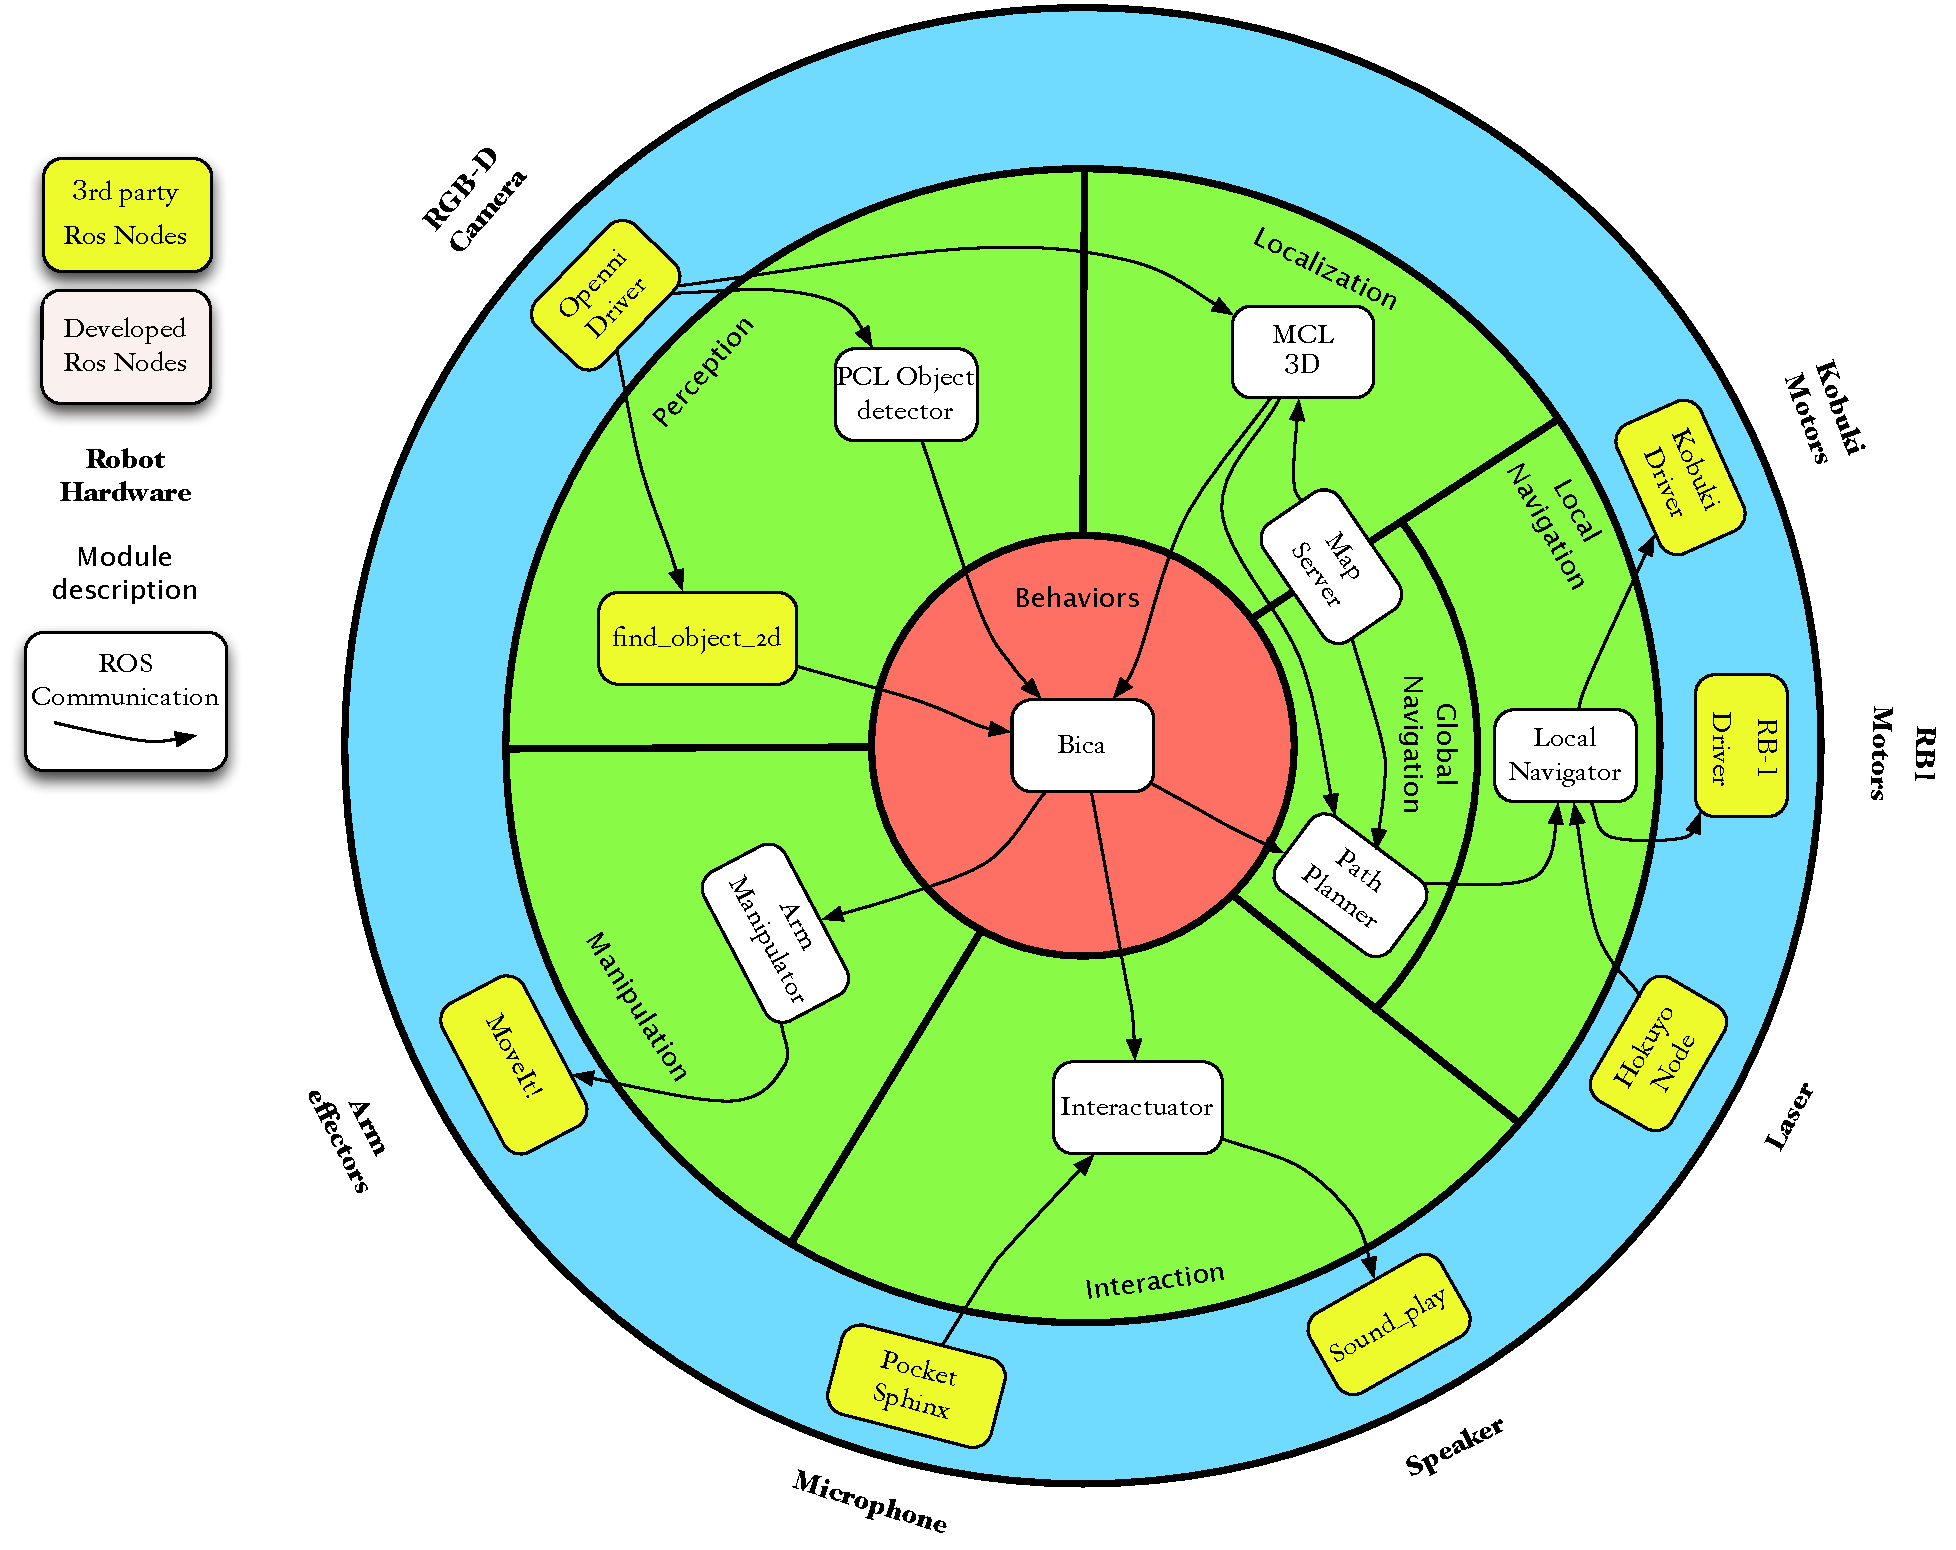
\includegraphics[width=0.8\textwidth]{rokinarq-142}
  \caption{Software architecture for RoCKIn competition.} 
  \label{fig:architecture}
\end{figure*}

\subsection{Architecture}

We have a three layers architecture based on ROS and Bica~\cite{aguero2010behavior}. 
The lower layer corresponds to ROS, and is in charge of hardware management. 
The intermediate layer provides the robot skills in order to carry out specific duties (perception, navigation,...).
The top layer presents Bica. It is a component-based for generating behaviour s architecture. This node coordinates the various
capabilities of the robot depending on the task to be carried out by the robot.
Figure~\ref{fig:architecture} shows the overall architecture of the software we have developed for participating in the RoCKIn competition. 
% In the peripheral layer, which represents the hardware access, we
% use third-party ROS nodes. In the intermediate layer, we have developed the skills that should
% have the robot to carry out their duties. Bica is at the core of this architecture. 







\subsubsection{Component-based behaviour  Architecture}

We use a component-based architecture~\cite{aguero2010behavior} to generate robot behaviour s. We recently
started the integration of this approach to our platform for avoiding big and complex finite
state machines (FSMs) developed ad-hoc in each ROS node. 

Figure~\ref{fig:BicaandROS} describes the implementation scheme of a robotic application using our approach.
There can be multiple ROS nodes containing components of our architecture, which communicate
with other ROS regular nodes. Besides ROS communications, ICE can be used to
interconnect any component with other processes or even to debug graphics applications.



\begin{figure}[ht!]
  \centering
  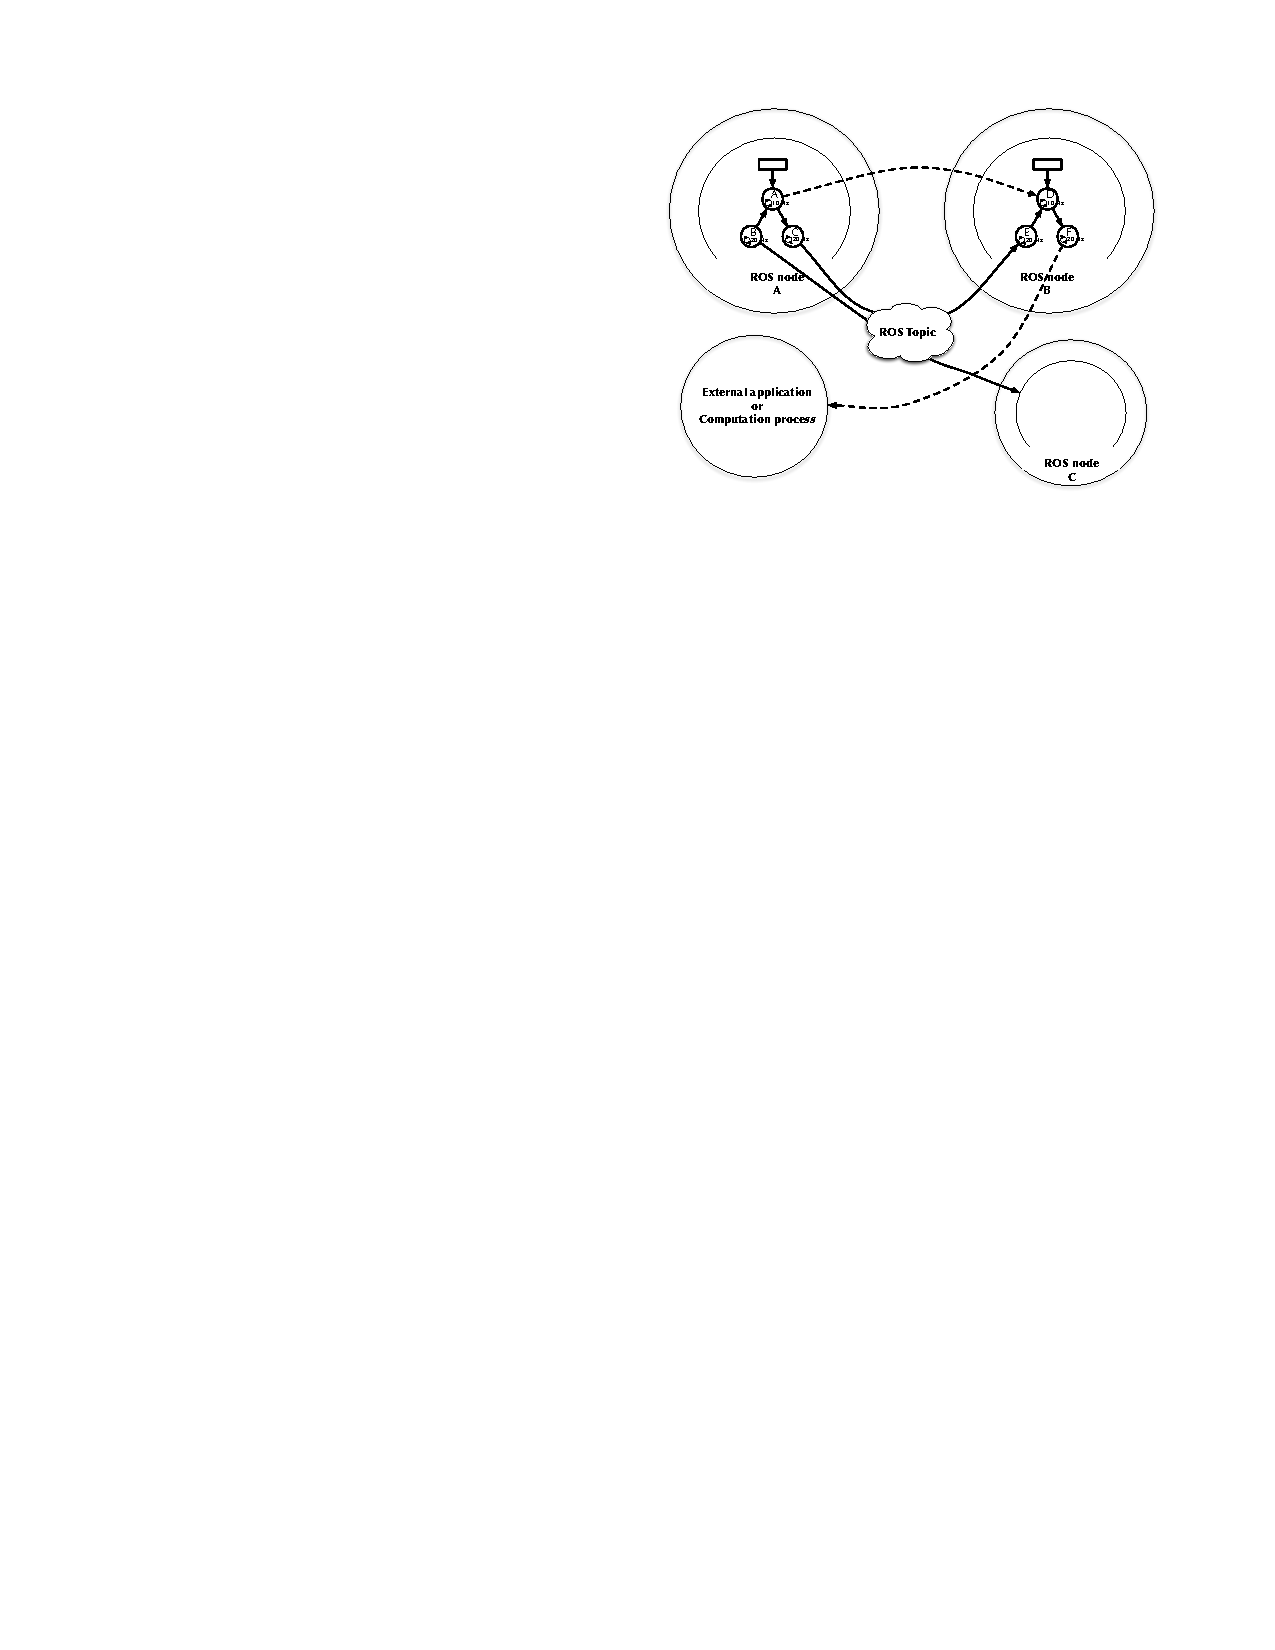
\includegraphics[width=0.5\textwidth]{50}
  \caption{Bica implementation inside ROS nodes. Solid lines represent ROS communication, and dashed lines ICE.} 
  \label{fig:BicaandROS}
\end{figure}




The basic functional unit in our architecture is the Component, simple functional units
that are executed iteratively at different rates. The main idea is to define components that
perform just a single task, but very efficiently. A running component can activate other
components, forming a dynamic hierarchy of components that implement a complete
behaviour .

Components can be very simple or very complex. Simple components communicate with
the underlying system methods to use sensors or motors, or some other components.
Complex components can be implemented as a FSM, so the set of components that are
activated depends of the current state.


Our approach uses only the required resources for a given task. When a component needs
another, it explicitly calls its step() method. Components that are not being used by
another component do not run, saving computing resources. 

We have developed a useful tool to design these complex components. This tool generates
the skeleton code for a behaviour  modelled graphically. Figure~\ref{fig:Bicacomponent} shows the implementation
of a component as an FSM with nine states (yellow circles). In each state, another component
(blue circles) are activated. From any component you can perform any communication with
other nodes ROS.


\begin{figure}[ht]
  \centering
  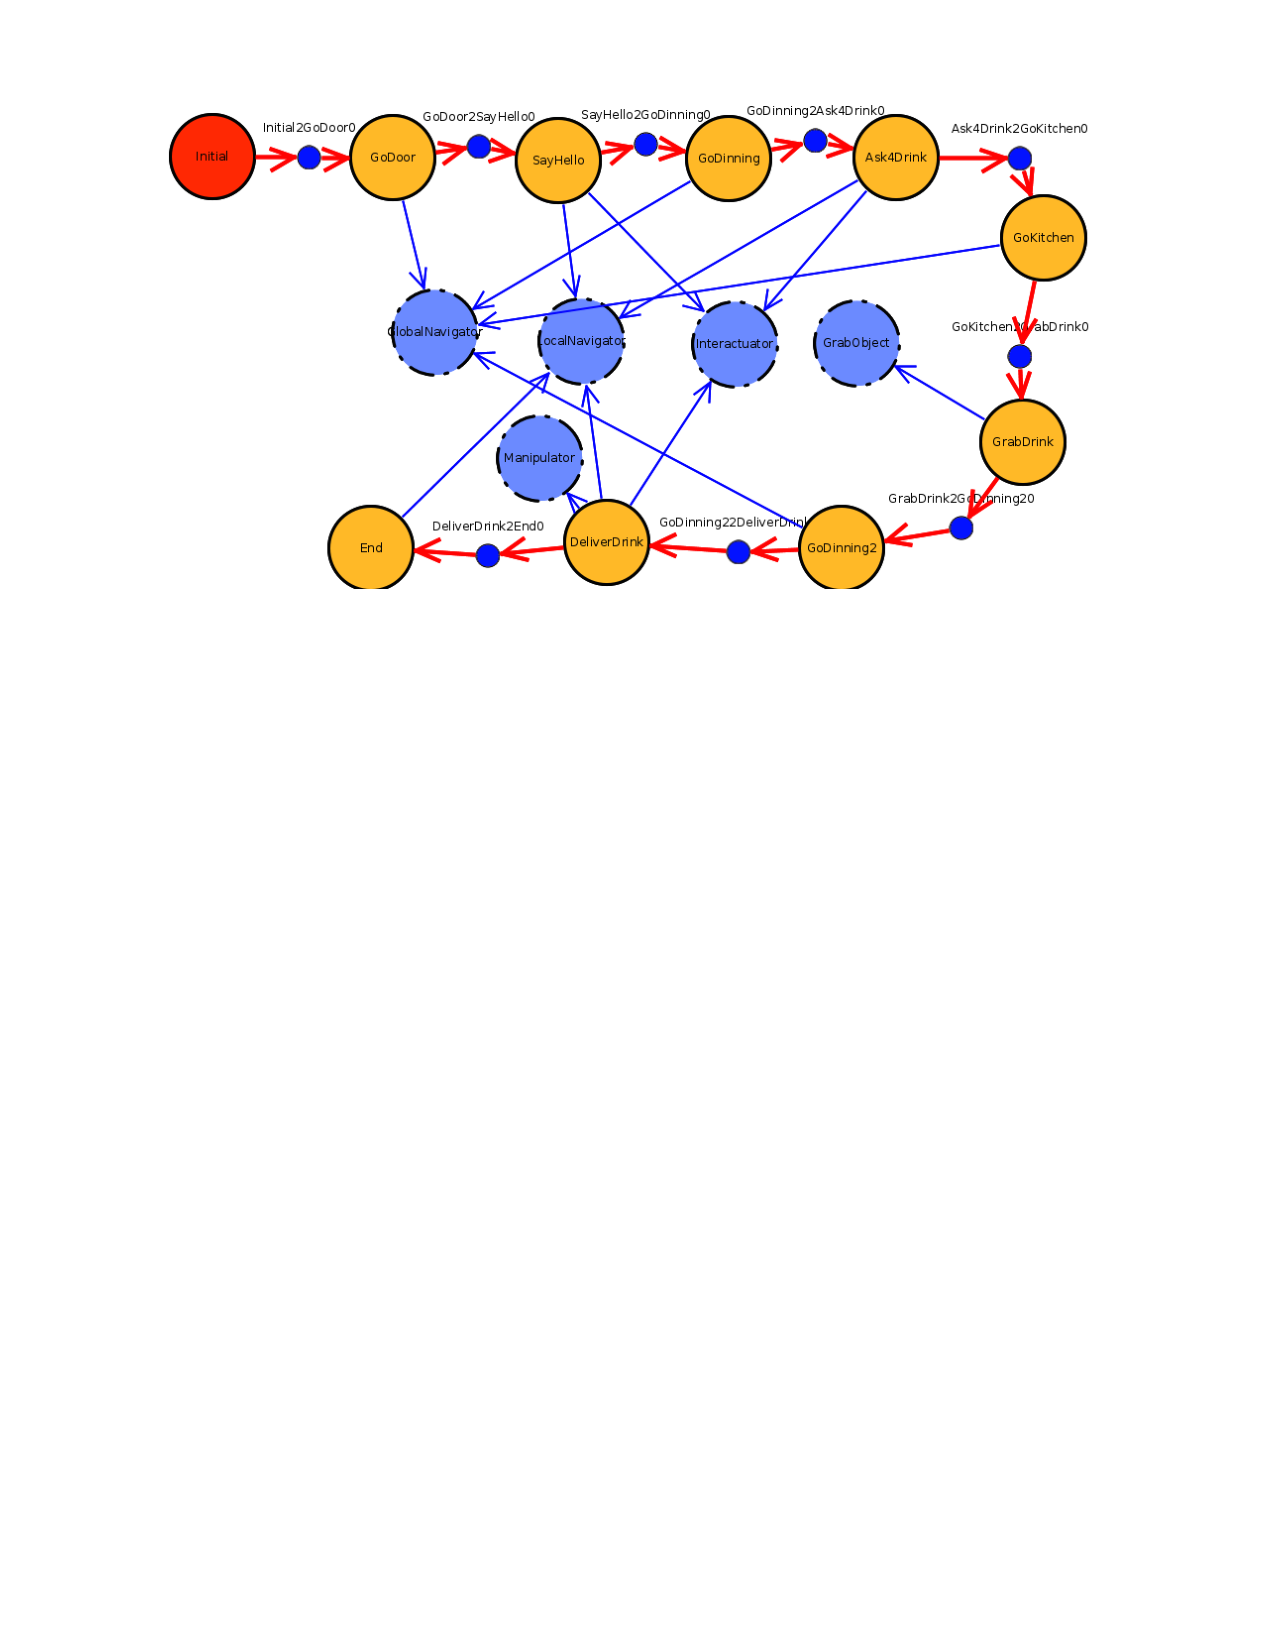
\includegraphics[width=0.5\textwidth]{202}
  \caption{Bica component implementing a finite state machine to define a high-level behaviour.} 
  \label{fig:Bicacomponent}
\end{figure}


\subsection{Perception}

We make intensive use of 3D perception. Both MYRABot as RB-1 are equipped with RGBD
Asus Xtion cameras. The position of each of the cameras is perfectly modeled by
transformations from its base, so that the result of perception is independent of the
platform used.

Apart from navigation tasks, the perception is used for the detection and recognition of
objects. For this task, we have used two alternatives. 

Our first approach was to use a  simple object detector called find\_object\_2D
developed by Mathieu Labbé~\cite{Mathieu2015}. This is ROS package that uses OpenCV with SIFT or SURF
descriptors and detectors, and it is 2D based only. This approach works well, although
it is focused on flat objects, not being suitable for estimating the position and
orientation of objects planes.

We have developed a new system for the Object Perception Functionality successfully tested last RoCKIn camp performed in Peccioli. 
This 3D solution uses PCL (Point Cloud Library) and a custom recognition
pipeline with global descriptors such as CVFH~\cite{aldoma2012our} to detect and classify objects in
segmented clusters. Objects are trained from CAD models, created by hand, using
multiple views.



\begin{figure}[ht]
  \centering
  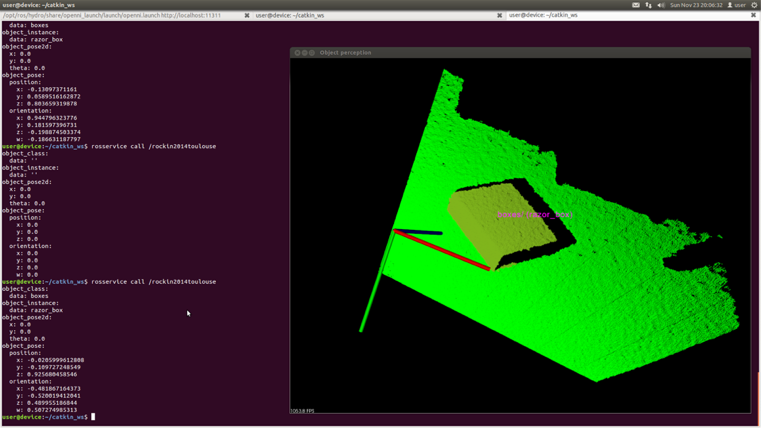
\includegraphics[width=0.5\textwidth]{Screenshot}
  \caption{Screenshot of our perception system running in lab environment.} 
  \label{fig:perception}
\end{figure}



\subsection{Navigation \& Mapping}

In previous editions of RoCKIn competition,  we have integrated the 2D navigation
stack from ROS\cite{tbd}. This package offers, among others, adaptive Monte Carlo Localization,
local and global planners, a costmap node for navigation, and a move base one that uses
Trajectory Rollout and Dynamic Window approach. 

% In Toulouse, we were able to run two
% demonstrations of simple robot behaviour  in the proposed home environment.

\begin{figure}[ht]
  \centering
  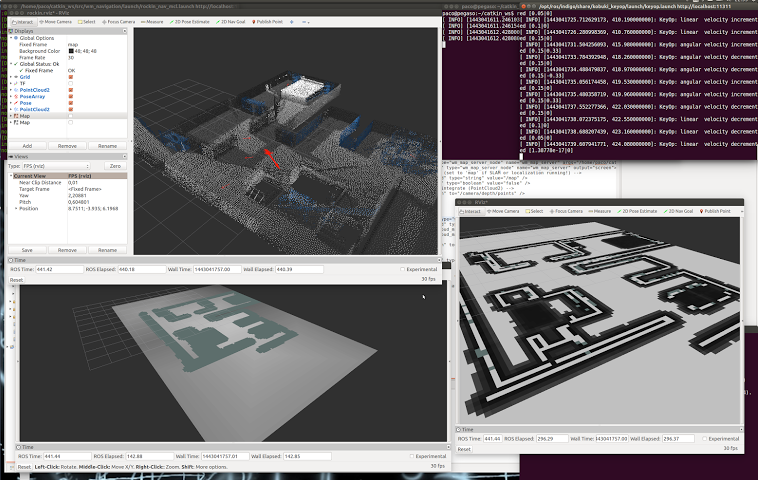
\includegraphics[width=0.5\textwidth]{Navigation}
  \caption{Rviz and Gazebo running the first approach of our 3D visual navigation method.} 
  \label{fig:navigation}
\end{figure}




For the next edition, we are planning to use our own self-localization algorithm based on
3D perception. Our approach consists of creating a 3D map of a cloud formed by RGB-D or
ColorOctomap \cite{hornung2013octomap} points. During operation of the robot, we will use an algorithm to
contrast the MCL RGB-D perception with the map to evaluate the population of particles.




\subsection{Manipulation}


Next RoCKIn we will use the RB-1 robot, which is equipped with a manipulator arm with 7 DOF. 
The arm mounts a gripper to perform manipulative interactions. With this kind of end-effector the manipulations task are limited to: grasping, lifting, pushing, pulling, placing and dropping. The lifting related tasks can be applied to objects up to 1kg of weight. 

The robot was designed to perform torso height adjustments.  
We have performed different manipulation experiments in order to analyze the right torso height for developing the functionalities in an assistance environment. These experiments have included both perception and grasping steps for  measuring the performance of the manipulation task. Figure~\ref{fig:RB1arm} shows one of these experiments. 

% Our main conclusion to these experiments is that this adjustments are great to perform any assistive task, but its performance is degraded 


% This arm includes a robotic hand with three fingers, allowing better manipulation of objects.

% 
% 
\begin{figure}[ht]
  \centering
  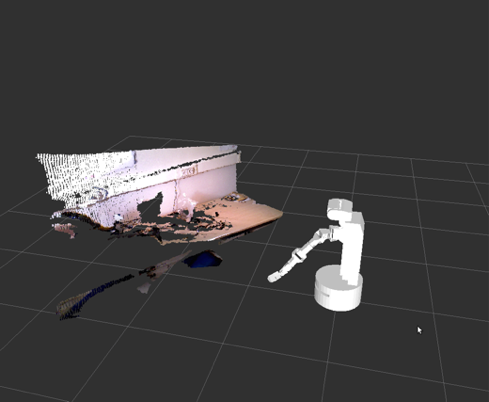
\includegraphics[width=0.4\textwidth]{199}
  \caption{Screenshot of Rviz application during the RB1 manipulator experiment.} 
  \label{fig:RB1arm}
\end{figure}



\subsection{Dialogue System}

The verbal human-robot interaction is performed under the same circumstances than previous challenges. 
However, we have changed our Automatic Speech Recognition software. 
We have changed the PocketSphinx solution to Sphinx solution due to its good performance in offline recognition tests.

% The architecture developed for the HRI is presented in figure 6. 
Now, our dialogue system is made up by three components. 
\begin{enumerate}
 \item Automatic Speech Recognition Component (ASR): This component is in charge of translating spoken words into text. 
 The system uses the CMU Sphinx Open Source Speech Recognition Toolkit, in particular the PocketSphinx engine for online speech recognition and Sphinx for offline recognition. 
  The key points of  CMU Sphinx solutions are: a)  The ASR should be speaker-independent,  and b) The speech recognition should have a well-defined vocabulary corpus directly related with the context, in our case the RoCKIn tasks
  \item Voice generator Component (VG): This component binds with the Festival library. The Festival solution is a speech synthesis system that offers a general framework for building speech synthesis systems. It is multi-lingual but we only use the English voice
package. 
\end{enumerate}



\section{RoCKIn Plan}
\label{sec:rockinplan}

\subsubsection{Hardware Specification:}

RoCKIn2015 is the first competition for RB1 robot. Its features fits with the ``General Specifications and Constraints on Robots and Teams'' proposed by RoCKIn committee. 

The platform characteristics as size or weight allow its deployment  in a home-like environment. 
It accomplishes the rulebook restriction of ``Safety Check'' integrating the “Emergency-Stop” button (figure~\ref{fig:button}). This mechanism will be used if the referee perceives that a robot has a potential to hurt an individual or cause harm to home  assets. When someone triggers this button, the system cuts the power to all joints of our platform. Under these circumstances, the robot can be moved (pushed) by team members to the area outside  the RoCKIn arena.

\begin{figure}[ht]
  \centering
  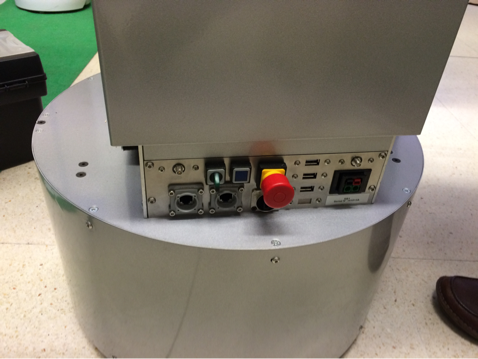
\includegraphics[width=0.3\textwidth]{111}
  \caption{Emergency-Stop button.} 
  \label{fig:button}
\end{figure}


\subsubsection{Benchmarks}

We are going to take part in the three functionality benchmarks proposed by RoCKIn: 
object perception, navigation and speech understanding. 
In addition we are working to participate in two of the functionality benchmarks proposed by RoCKIn: 
welcoming visitors, and catering for Granny Annie's comfort. 


% An example of a floating figure using the graphicx package.
% Note that \label must occur AFTER (or within) \caption.
% For figures, \caption should occur after the \includegraphics.
% Note that IEEEtran v1.7 and later has special internal code that
% is designed to preserve the operation of \label within \caption
% even when the captionsoff option is in effect. However, because
% of issues like this, it may be the safest practice to put all your
% \label just after \caption rather than within \caption{}.
%
% Reminder: the "draftcls" or "draftclsnofoot", not "draft", class
% option should be used if it is desired that the figures are to be
% displayed while in draft mode.
%
%\begin{figure}[!t]
%\centering
%\includegraphics[width=2.5in]{myfigure}
% where an .eps filename suffix will be assumed under latex, 
% and a .pdf suffix will be assumed for pdflatex; or what has been declared
% via \DeclareGraphicsExtensions.
%\caption{Simulation results for the network.}
%\label{fig_sim}
%\end{figure}

% Note that IEEE typically puts floats only at the top, even when this
% results in a large percentage of a column being occupied by floats.


% An example of a double column floating figure using two subfigures.
% (The subfig.sty package must be loaded for this to work.)
% The subfigure \label commands are set within each subfloat command,
% and the \label for the overall figure must come after \caption.
% \hfil is used as a separator to get equal spacing.
% Watch out that the combined width of all the subfigures on a 
% line do not exceed the text width or a line break will occur.
%
%\begin{figure*}[!t]
%\centering
%\subfloat[Case I]{\includegraphics[width=2.5in]{box}%
%\label{fig_first_case}}
%\hfil
%\subfloat[Case II]{\includegraphics[width=2.5in]{box}%
%\label{fig_second_case}}
%\caption{Simulation results for the network.}
%\label{fig_sim}
%\end{figure*}
%
% Note that often IEEE papers with subfigures do not employ subfigure
% captions (using the optional argument to \subfloat[]), but instead will
% reference/describe all of them (a), (b), etc., within the main caption.
% Be aware that for subfig.sty to generate the (a), (b), etc., subfigure
% labels, the optional argument to \subfloat must be present. If a
% subcaption is not desired, just leave its contents blank,
% e.g., \subfloat[].


% An example of a floating table. Note that, for IEEE style tables, the
% \caption command should come BEFORE the table and, given that table
% captions serve much like titles, are usually capitalized except for words
% such as a, an, and, as, at, but, by, for, in, nor, of, on, or, the, to
% and up, which are usually not capitalized unless they are the first or
% last word of the caption. Table text will default to \footnotesize as
% IEEE normally uses this smaller font for tables.
% The \label must come after \caption as always.
%
%\begin{table}[!t]
%% increase table row spacing, adjust to taste
%\renewcommand{\arraystretch}{1.3}
% if using array.sty, it might be a good idea to tweak the value of
% \extrarowheight as needed to properly center the text within the cells
%\caption{An Example of a Table}
%\label{table_example}
%\centering
%% Some packages, such as MDW tools, offer better commands for making tables
%% than the plain LaTeX2e tabular which is used here.
%\begin{tabular}{|c||c|}
%\hline
%One & Two\\
%\hline
%Three & Four\\
%\hline
%\end{tabular}
%\end{table}


% Note that the IEEE does not put floats in the very first column
% - or typically anywhere on the first page for that matter. Also,
% in-text middle ("here") positioning is typically not used, but it
% is allowed and encouraged for Computer Society conferences (but
% not Computer Society journals). Most IEEE journals/conferences use
% top floats exclusively. 
% Note that, LaTeX2e, unlike IEEE journals/conferences, places
% footnotes above bottom floats. This can be corrected via the
% \fnbelowfloat command of the stfloats package.




\section{Conclusions}
\label{sec:conclusions}
We have described the main characteristics of our team for the 2015 RoCKIn competition. 
We will attend this challenge with RB-1 platform.
This platform provides us a more stable platform to take part in competitions benchmarks than our previous low-cost robot MYRABot.
We have also presented the software novelties deployed in our platform. 
Our website maintains updated information about Watermelon Project team and our software development.


% conference papers do not normally have an appendix


% use section* for acknowledgment
\section*{Acknowledgments}

The research activities of our team are funded by: 
\begin{itemize}
 \item Grant DPI2013-40534-R of Spanish Ministry of Economy and Competitiveness "Development of an integral robotic system for surveilling and interaction
with dependents and people suffering acquired brain injury” (SIRMAVED).
\item C\'atedra Telef\'onica for TIC and Society Ageing.
\item University of Le\'on
\end{itemize}



% trigger a \newpage just before the given reference
% number - used to balance the columns on the last page
% adjust value as needed - may need to be readjusted if
% the document is modified later
%\IEEEtriggeratref{8}
% The "triggered" command can be changed if desired:
%\IEEEtriggercmd{\enlargethispage{-5in}}

% references section

% can use a bibliography generated by BibTeX as a .bbl file
% BibTeX documentation can be easily obtained at:
% http://www.ctan.org/tex-archive/biblio/bibtex/contrib/doc/
% The IEEEtran BibTeX style support page is at:
% http://www.michaelshell.org/tex/ieeetran/bibtex/

%   \bibliographystyle{unsrt}
\bibliographystyle{IEEEtrans}
% argument is your BibTeX string definitions and bibliography database(s)
\bibliography{biblio}
%
% <OR> manually copy in the resultant .bbl file
% set second argument of \begin to the number of references
% (used to reserve space for the reference number labels box)
% \begin{thebibliography}{1}
% 
% \bibitem{IEEEhowto:kopka}
% H.~Kopka and P.~W. Daly, \emph{A Guide to \LaTeX}, 3rd~ed.\hskip 1em plus
%   0.5em minus 0.4em\relax Harlow, England: Addison-Wesley, 1999.
% 
% \end{thebibliography}




% that's all folks
\end{document}


